\begin{Exemple}[Organiser vscode]

    Une fois configuré, votre environnement de travail devrait ressembler à ceci : 

    \begin{center}
        \begin{tikzpicture}
            % Image de base
            \node[anchor=center, inner sep=0] (image) at (0,0) {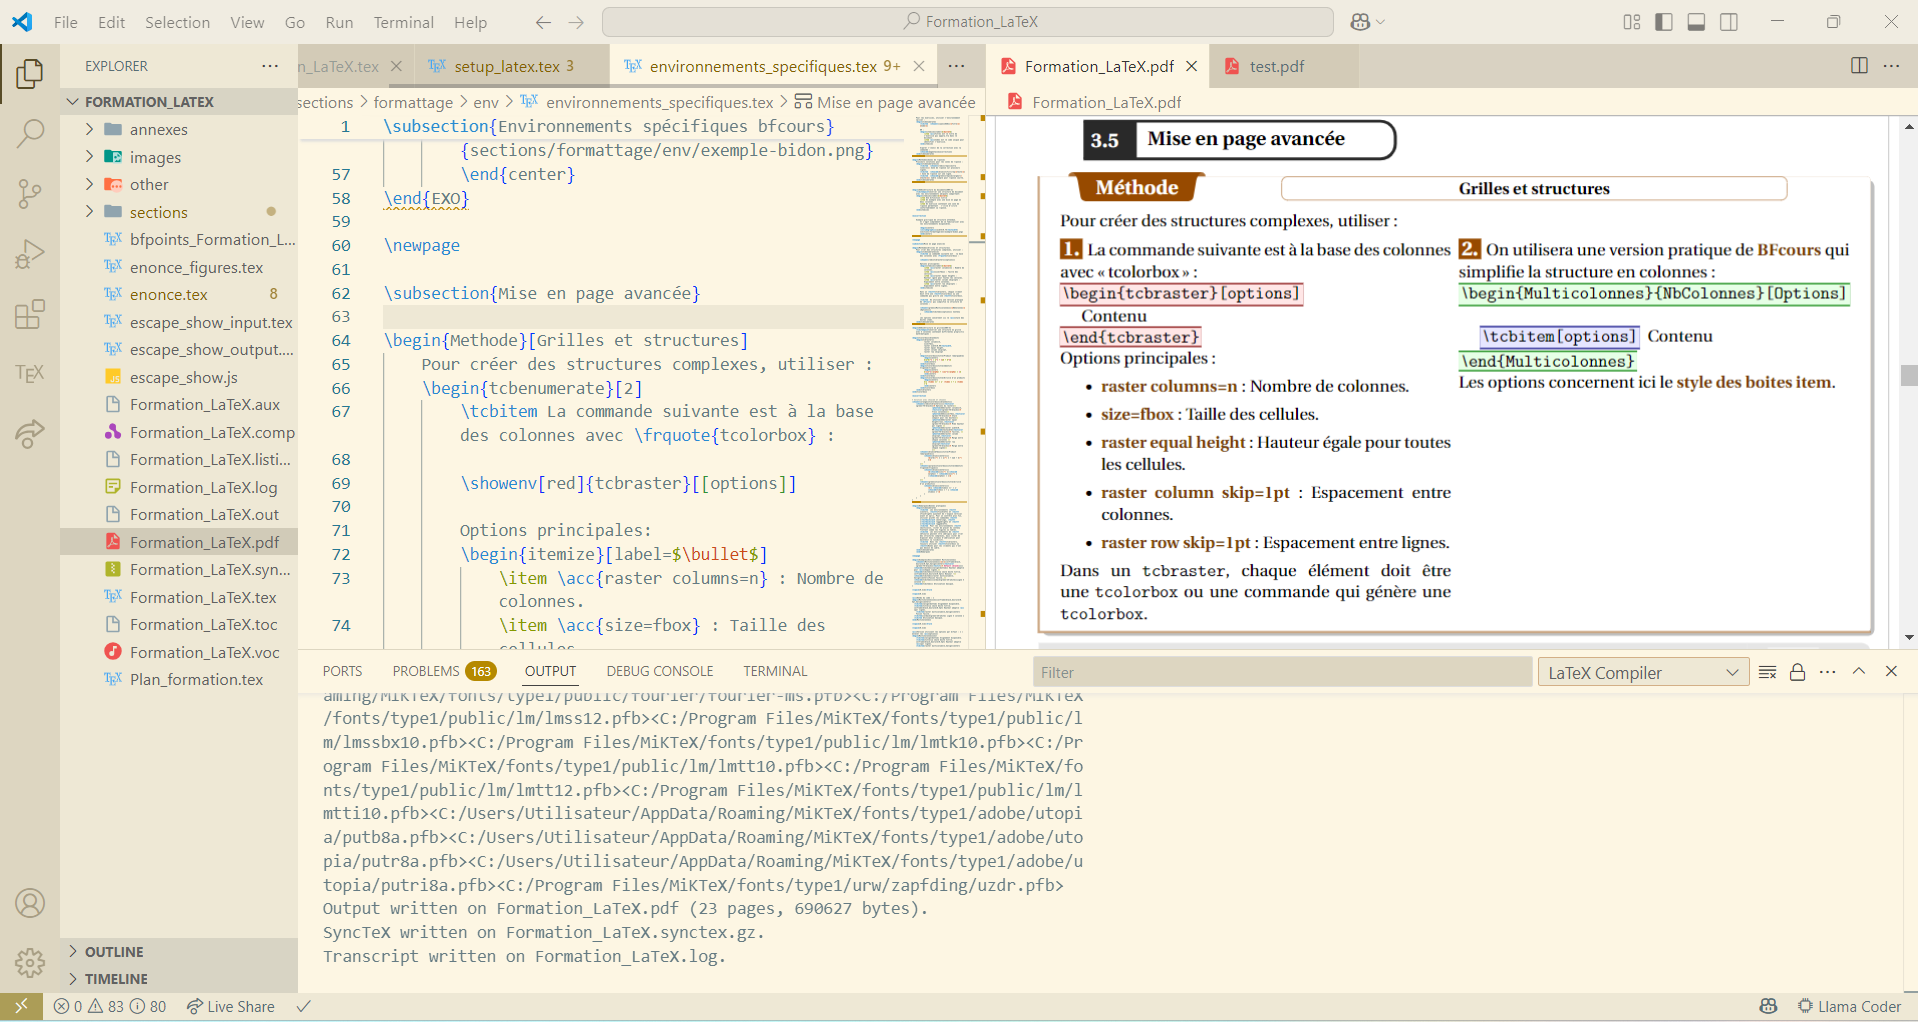
\includegraphics[width=0.8\textwidth]{images/IDE/VSCode_use.png}};
            
            % Obtenir les dimensions de l'image
            \pgfgetlastxy{\maxx}{\maxy}
            
            % Style pour les pastilles
            \tikzset{
                pastille/.style={
                    circle, 
                    fill=red!90!black, 
                    text=white, 
                    font=\bfseries\footnotesize,
                    minimum size=20pt,
                    inner sep=0pt,
                    draw=white,
                    line width=1.5pt
                }
            }
            
            % Placement des pastilles (positions relatives à l'image)
            % 1. Options générales - coin supérieur gauche
            \node[pastille] at (-7, 3.7) {1 $\rightarrow$};
            
            % 2. Barre de recherche - centre haut
            \node[pastille] at (0, 3.8) {2};
            
            % 3. Géométrie voulue pour le terminal - bas
            \node[pastille] at (4.2, 3.7) {3};
            
            % 4. La sidebar - gauche
            \node[pastille] at (-7, 0.5) {4 $ \uparrow $};
            
            % 5. Zone d'exploration - gauche dans la sidebar
            \node[pastille] at (-6, 1.5) {5};
            
            % 6. Onglets - haut du contenu principal
            \node[pastille] at (-2, 3) {6};
            
            % 7. Zone de saisie principale - centre
            \node[pastille] at (-2.5, 0) {7};
            
            % 8. Zone d'affichage secondaire - droite
            \node[pastille] at (3.5, 0) {8};
            
            % 9. Terminal - tout en bas
            \node[pastille] at (0, -2.2) {9};
        \end{tikzpicture}
    \end{center}

    On observe : 
    \begin{tcbenumerate}[2]
        \tcbitem Options générales
        \tcbitem Barre de recherche
        \tcbitem Géométrie voulue pour le terminal
        \tcbitem La \acc{sidebar}
        \tcbitem La zone d'exploration ( fichiers, extensions, recherche sur fichiers multiples )
        \tcbitem Onglets
        \tcbitem Zone de saisie principale
        \tcbitem Zone d'affichage ou de saisie secondaire
        \tcbitem Terminal - permet également d'afficher les logs : 

        \bouton{OUTPUT}$\rightarrow$\bouton{Latex Compiler}
    \end{tcbenumerate}
\end{Exemple}